\section{Simulation}
\label{sec:simulation}
In order to analyze the effectiveness of a time analysis attack in a
realistic scenario, we decide to consider a simulation environment.
We wanted to model the scenario in a way that most of the
characteristics of the Tor network architecture would have been
considered.

The \textbf{shadow simulator}\cite{shadow} seemed to be a good candidate for our purpose. In
the next paragraphs we will introduce shadow and we will illustrate our
work based on this simulator.
 
\subsection{Shadow}
\label{sec:Shadow}
Most of the simulators used for networks experimentation do not provide
the use of real external applications, which their
behaviour are often simulated as well. 
This approach can be reasonable if the analysis is focused on the 
network layers below the application layer. 

In our case we are interested in studying the characteristic of the Tor
network which is based on the network application layer.
Thus the Tor application is one of the core part of the Tor architecture as it implements the
onion routing protocol that let the Tor nodes communicate each others.

It is evident that the Tor application has a significant role in
the Tor architecture, thus we chose the shadow simulator as it permits
the use of the real Tor applications in a simulated environment.
Essentially it allows the execution of a set of local applications that
communicates in a simulated computer network. Moreover we could
avoid the oversimplification of the system that could have been occurred
with a custom implementation.

Applications are executed inside the shadow simulator through 
dynamic libraries called plug-ins. 
These plug-ins are interfaces used by shadow to trace a
selective set of system functions and re-route them to the simulator instead
of letting them proceed directly to the kernel. 
In this way, the simulator is transparent to the application
that may function as like it was running in a standard UNIX environment. 

The plug-in that allows the execution of the Tor applications is
scallion. The latter provides also some useful tools for the virtual
Tor network topology generation.

The virtual network is modeled with a XML configuration
file, called blueprint, used by shadow to understand the network
structure and some network properties such as link latency, jitter and
packet loss rate. The blueprint also tells Shadow what software each
virtual node should run at its creation. This is specified with a
plug-ins list for each virtual node entry of the XML file.

We implemented three shadow plug-ins and their relative applications 
 able to work alongside scallion in
order to experiment a time analysis attack scenario. Our plug-ins and
the attack scenario will be illustrated in the next paragraphs.

%TODO: find some pictures
\subsection{Simulation Scenario}
\begin{figure}[H]
    \centering
    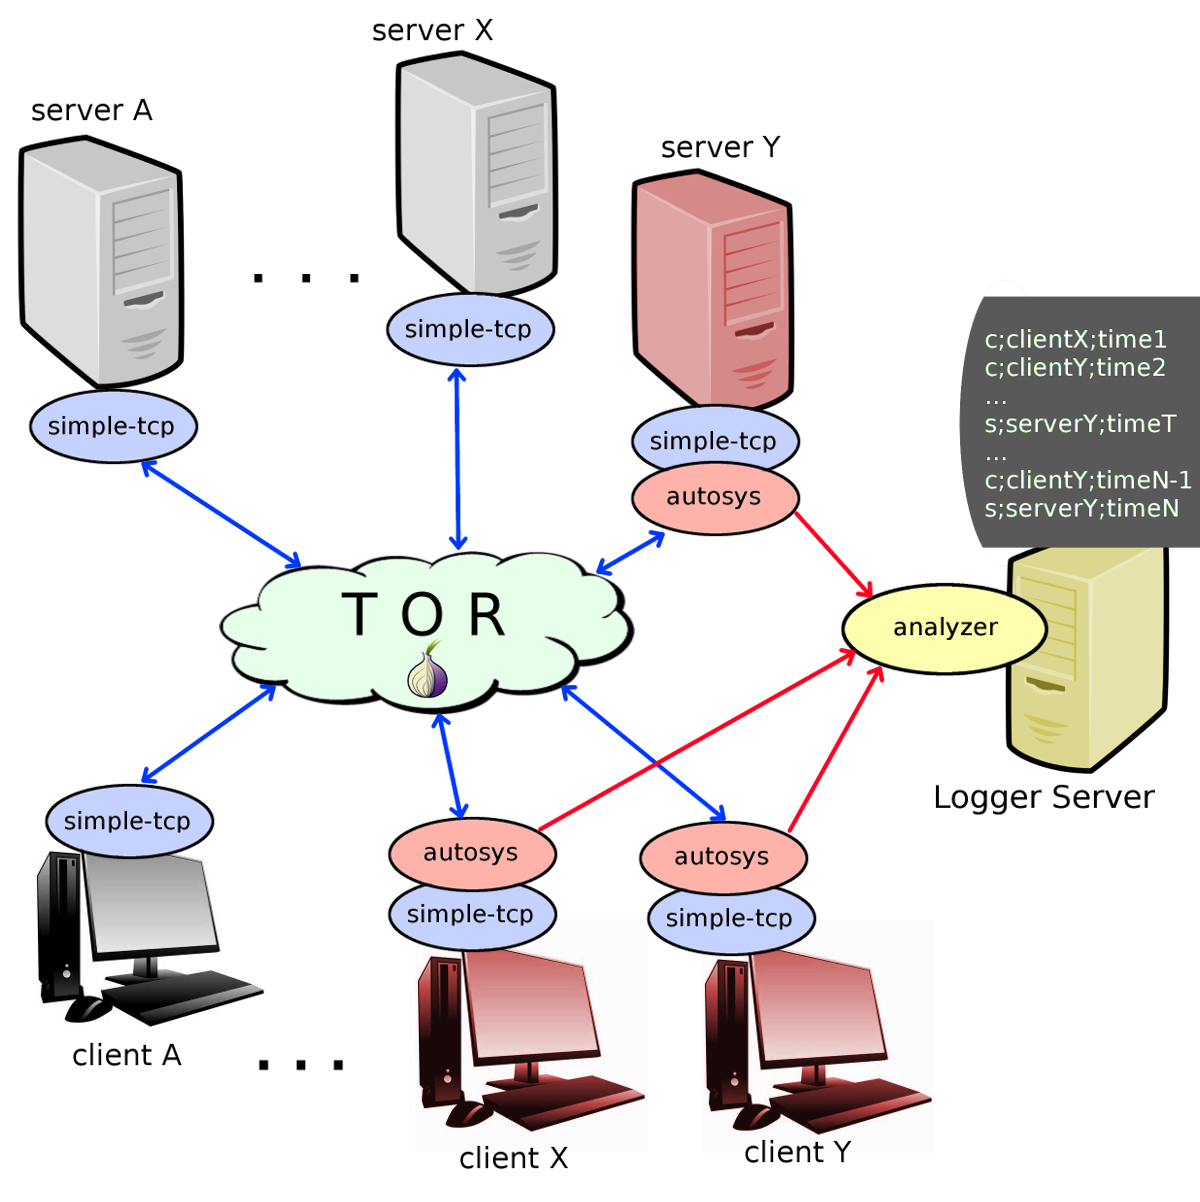
\includegraphics[scale=0.33]{scenario.png}
    \caption{Time analysis attack simulation scenario.}
    \label{fig:scenario}
\end{figure}

The figure \ref{fig:scenario} shows an outline of the simulation
scenario. More specifically the considered identities of the scenario are:
\begin{itemize} 
	\item \textbf{Servers}, that represent usual application servers.
They listen on some TCP port waiting for connection requests.
	\item \textbf{Clients}, that represent usual application clients.
They try to initialize TCP connections with some servers through the
destination port the target servers are listening to.
	\item \textbf{Tor nodes}, that form Tor communication paths. They
compose the Tor network.
	\item \textbf{Logger server}, that is a simple server whose read
and store incoming UDP status messages.
\end{itemize}

Furthermore, clients and servers communicate each others at the application layer
through an ad-hoc application we built, \textbf{simple-tcp}. As the
application name itself suggests, simple-tcp permits clients to
establish simple TCP connections with servers. Also, simple-tcp is used
by clients to send their own IP address to the servers in the TCP
messages payload.
In this way servers can log some information about the incoming connections:
specifically they store source IP address,
destination IP address and time of day related to them. 
This feature is not intended to be used by an attacker but
we will see in the paragraph \ref{subsec:simpletcp} how
it is useful in the analysis process. Anyway, from the attacker point of
view, simple-tcp tries to behave like an usual web-application,
simulating a sequence of TCP connections interchange between clients and
servers. 

In our scenario all the TCP connections pass through the Tor
nodes as we are not interested in the traffic outside the Tor network. 
This is legitimated considering our purpose of testing the feasibility of a time analysis
attack in Tor and considering that the internet traffic coming from
outside Tor could be filtered by the attacker's tracer
software\footnote{The Tor exit nodes list is public\cite{torstatus}.}, avoiding in this
way unwanted data interference.

As a simplification of the implementation we decided that during a
simulation a client is able to
request several TCP connections to a single server only. 
An extension of the application that allows a client to connects to more servers may be
implemented in future. Anyway this limitation is for now negligible if we
consider that a client usually requests a large amount of HTTP fragments and TCP
connections to the same
domain in a certain temporal window. Hopefully this assumption should
suggest similar results considering client applications with multi-server
requests but this is indeed a critical point to be tested in future
works.
\textbf{Autosys} is a tracer application installed on both clients and
servers which are interesting for an attacker.  
In short, when autosys discover an outgoing connection from the
hosting client, it sends to a logger server the client IP address and
the current time of day. Doing the same when it discovers incoming
connections in the server side, autosys may let the attacker relate outgoing
clients connections 
 to incoming server connections. We will see in the next
paragraph how this application can be used to simulate a time analysis
attack.
\subsection{Autosys plug-in}
To analyze the tor network traffic we need, at least, some information about
the incoming and the outgoing connections.\\
To achieve this result we have more than a solution: in the first one we can place 
in the last network element that is under the control of an \textbf{autonomous system}\footnote{
That the reason why the plug-in is called "Autosys".} a connection
listener which traces a whole subset of
network nodes;
otherwise we can place the listener in a, malware-like, invisible proxy on the target
machine with the aim to trace every outgoing connection. 
In both solutions we need to place some correspondent exit tracers on
the target end points.
This proxies can be implemented as a simple raw-socket based sniffer. 
Unfortunately Shadow doesn't support raw-socket
emulation\footnote{If you launch a simulation with a raw socket based program the simulator
inform you about the impossibility of the task.},
so we implemented the plug-in as a simple event based TCP
proxy. In our attack scenario an instance of the autosys plug-in is placed 
between the client application and the client Tor daemon, also a second
 instance is placed between the server Tor daemon and the server application.
\\
\begin{algorithm}
\caption{Autosys main loop}
\begin{algorithmic}[1]
\Function{Autosys}{$sa$, $sb$, $analyzer$}
	\While{$True$}
		\If {Some data can be read from $sa$}
			\State $indata \gets $ readall($sa$)
			\State writeall($sb$, $indata$)
			\If {$indata$ was a connection initiator}
				\State send($<type(sa)$;$hostname(sa)$;$gettod()>$, analyzer)
			\EndIf
		\EndIf
		\If {Some data can be read from $sb$}
			\State $indata \gets $ readall($sb$)
			\State writeall($sa$, $indata$)
			\If {$indata$ was a connection initiator}
				\State send($<type(sa)$;$hostname(sa)$;$gettod()>$, analyzer)
			\EndIf
		\EndIf
	\EndWhile
\EndFunction
\end{algorithmic}
\label{alg:auto_main}
\end{algorithm}

As we can see in the algorithm \ref{alg:auto_main}, where $sa$ and $sb$ are the two end sockets and
$analyzer$ is the socket descriptor of the \textbf{analysis server} (the logger), when some connection
initiator packets flow trough the proxy the
current machine time of day is sent to the \textbf{analysis server}
%TODO DA CONTROLLARE FOOTNOTE
\footnote{The simulator have a single clock, so we don't have any problem with the
clock synchronization.}.

\begin{figure}[H]
\centering
\begin{tikzpicture}[scale=2]
\node (app) [rectangle, draw, thick, rounded corners=3pt, text width=100pt, fill=blue!50]{Application};
\node (autosys) [rectangle, draw, thick, rounded corners=3pt, text width=100pt, fill=red!50, below = 0.5cm of app]{Autosys};
\node (tor) [rectangle, draw, thick, rounded corners=3pt, text width=100pt, below = 0.5cm of autosys]{\begin{center}TOR daemon\\
\includegraphics[scale=0.3]{tor.jpg}\end{center}};

\node (internet) [cloud, draw, thick, fill=red!20!blue!20!green!20, right = 2 cm of tor] {Net};

\node (analysis) [rectangle, draw, thick, rounded corners=3pt, text width = 100pt, below= 1cm of internet, fill=yellow!50] {Logger};

\node (server) [rectangle, draw, thick, rounded corners=3pt, text width = 100pt, right = 2cm of internet, fill=blue!50] {Server};


\draw [thick] (app) -- node [left] {localhost:10000} (autosys);
\draw [thick] (autosys) -- node[left] {localhost:9050} (tor);

\draw [thick, color=blue]  (tor) -> (internet) {};
\draw [thick, color=blue]  (internet) -> (server) {};
\draw [thick, color=red]   (autosys) -| (internet) {};
\draw [thick, color=red]   (internet) -- node [right]{Tracker packet} (analysis);
\end{tikzpicture}
\caption {Autosys proxy structure.}
\label{fig:autosys_diagram}
\end{figure}

\subsection{Analyzer plug-in}
Data sniffed by the \textbf{autosys} plug-in need to be stored for later analysis, 
to do so we need another plug-in.
This plug-in is called the "Analyzer plug-in", "Analysis server" or
simply "Logger"
which will collect all the dead-drops generated by the sniffers.
The plug-in is implemented as a simple event driven UDP server, every
packet received from the sniffer plug-in is so saved in a single place.
\begin{figure}[H]
\begin{lstlisting}[language=bash,frame=single]
host_type;hostname;timestamp
\end{lstlisting}
\caption{Analyzer log Structure}
\label{fig:analyzer_pack_struct}
\end{figure}
Referring to the figure \ref{fig:analyzer_pack_struct} we have the following
information in the log:
\begin{itemize}
\item Host Type \hfill \\
\emph{c} to signal that the traced packet referred to a client\\
\emph{s} to signal that the traced packet referred to a server
\item Hostname \hfill \\
The name of the tracked machine
\item Timestamp \hfill \\
The time-stamp of the packet (when it flows trough the autosys plug-in).
\end{itemize}

In conclusion this raw data will be passed to the phase two to be analyzed by the scripts.\\
\begin{figure}[H]
\centering
\begin{tikzpicture}[scale=2]
\node (internet) [cloud, draw, thick, fill=red!20!blue!20!green!20] {Net};
\node (analysis) [rectangle, draw, thick, rounded corners=3pt, text width = 100pt, below= 1cm of internet, fill=yellow!50] {Logger};

\pic(disc2) [
	draw,
	below = 1.7cm of analysis,
	scale = 0.5
] {disc};
\pic(disc1) [
	draw,
	below = 1.1cm of analysis,
	scale = 0.5
] {disc};
\pic(disc0) [
	draw,
	below = 0.5cm of analysis,
	scale = 0.5
] {disc};


\draw [thick, color=red]   (internet) -- node [right]{Tracker packet} (analysis);
\draw [thick, color=red]   (analysis) -- (0,-1.37);
\end{tikzpicture}
\caption {Logger logic structure.}
\label{fig:autosys_diagram}
\end{figure}

As a subnote this plug-in was implemented as an UDP server for the sake of
simplicity and, in opposite to TCP, the low impact on the network.\\
This can lend us to a little packet-loss but won't impact too much on the time analysis
as we will see later on this study.

\subsection{Simpletcp plug-in}
\label{subsec:simpletcp}
The last plug-in that we implemented emulate a simple HTTP client/server communication,
this plug-in have two operational modes: the client mode and the server mode.
\subsubsection {Client mode}
\label{sec:simpletcpclient}
This plug-in, in client mode, emulate the communication making some (a customizable amount)
connections to the server
with a random uniform distribute sleep time in between of every connection
(this parameter is configurable too).\\
The packet transfered by the plug-in simply contains the host-name of the
host machine, this is to break the anonymity of the TOR system and analyze the results
in later phases.\\
\subsubsection {Server mode}
At the opposite end, a server \textbf{simpletcp} instance, will:
\begin{itemize}
	\item Receive the connection packets from the clients.
	\item Add a time-stamp to the current received packet.
	\item Save the packet to a common file (in our implementation this data
	file is called as the host-name of the machine hosting the server).
	This is used in the analysis of the phase 2, to compute a matching probability
	between the guessed users and the real users.
\end{itemize}


\subsubsection {SOCKS5 operation}
To communicate over TOR we implemented the \textbf{simpletcp} plug-in as a \textbf{SOCKS5} capable
client.\\
The \textbf{SOCKS5} proxies works as described in the RFC1928\cite{leech1996rfc},
in a nutshell the \textbf{SOCKS5} is a transparent proxy design, it describe an establishment
phase in which the proxy is informed about the other host, make the outgoing connection
and, when some data is written on the incoming connection (from the client)
the proxy will transmit this data trough the outgoing connection.\\

\begin{figure}[H]
\centering
	\begin{sequencediagram}
		\newthread{c}{Client}
		\newinst[4]{p}{SOCKS5 Proxy}
		\newinst[4]{s}{Server}

		\begin{sdblock}{Connection establishment}{}
		\begin{call}{c}{Connection request}{p}{}
		\begin{call}[3]{p}{Connection}{s}{}
		\end{call}
		\end{call}
		\end{sdblock}

		\begin{sdblock}{Normal Communication}{}
		\begin{call}{c}{}{s}{}
		\end{call}
		\end{sdblock}

		\begin{sdblock}{Connection teardown}{}
		\begin{call}{c}{Connection Close}{p}{}
		\end{call}
		\end{sdblock}

	\end{sequencediagram}
\caption{Socks5 Proxy behaviour}
\end{figure}

This proxy-like approach is required because the
TOR interface is implemented as a \textbf{SOCKS5} proxy, when some packet flows
trough the interface (which is listening by default on \textbf{localhost} on port 9050)
the TOR daemon will transmit over the TOR network following the anonymity methods
described in the previous chapters.

\subsection{Summary}

\begin{figure}[H]
	\begin{sequencediagram}
		\newthread{stc}{SimpleTcp}
		\newinst{ac}{Autosys}
		\newinst{tc}{TOR daemon}
		\newinst[1]{ts}{TOR exit node}
		\newinst[1]{as}{Autosys}
		\newinst{sts}{SimpleTcp}
		\newinst[1]{log}{Logger}

		\begin{call}{stc}{}{ac}{}
			\mess{ac}{Trace}{log}
			\begin{call}{ac}{}{tc}{}
			\begin{call}{tc}{...TOR...}{ts}{}
			\begin{call}{ts}{}{as}{}
			\mess{as}{Trace}{log}
			\begin{call}{as}{}{sts}{}
			\end{call}
			\end{call}
			\end{call}
			\end{call}
		\end{call}
	\end{sequencediagram}
\label{fig:simpletcpsummary}
\caption{Summarization of the behaviour of the plug-ins system (only one connection of the simpleTcp plugin)}
\end{figure}
